% Compile with pdfLaTeX, twice. All figures and the NeurIPS 2025 style are bundled.
% Repository URL supplied by the group and included in the abstract footnote.
\documentclass{article}
\usepackage[preprint,nonatbib]{neurips_2025}
\usepackage[T1]{fontenc}
\usepackage[utf8]{inputenc}
\usepackage{amsmath,amssymb,bm,booktabs,array,tabularx,multirow}
\usepackage{graphicx,xcolor,url,microtype}
\usepackage[numbers,sort&compress]{natbib}
\usepackage{enumitem,float,placeins,fancyvrb}
\usepackage{hyperref}
\hypersetup{colorlinks=true,linkcolor=black,citecolor=black,urlcolor=blue,
  pdftitle={Cost-Sensitive SVM for Credit Card Fraud Detection},
  pdfauthor={Group 4}}
\newcommand{\RepositoryURL}{https://github.com/xiaoxiaoxiaotao/PolyU-COMP6704-Group4}
\newcommand{\repositorynote}{Code repository: \expandafter\url\expandafter{\RepositoryURL}.}
\makeatletter
\renewcommand{\@noticestring}{COMP6704 Advanced Topics in Optimization, Group 4, The Hong Kong Polytechnic University, Fall 2026.}
\makeatother
\newcommand{\hinge}[1]{\left[#1\right]_{+}}
\newcommand{\R}{\mathbb{R}}
\newcommand{\ind}{\mathbf{1}}
\newcommand{\FN}{\mathrm{FN}}
\newcommand{\FP}{\mathrm{FP}}
\newcommand{\FNcost}{c_{\mathrm{FN}}}
\newcommand{\FPcost}{c_{\mathrm{FP}}}
\newcommand{\pref}{P_{\mathrm{ref}}}
\setlist{nosep,leftmargin=1.4em}
\setlength{\emergencystretch}{1em}
\raggedbottom

\title{Cost-Sensitive SVM for Credit Card Fraud Detection\\
Comparing Convex Optimization Methods}
% Author names and student identifiers are deliberately absent from this file.
% They live in groupauthors.tex, which git ignores. With that file present the title
% page prints the real authors (the Canvas submission build); without it the build says
% "Group 4" (the public repository build). No tracked file names anyone.
\IfFileExists{groupauthors.tex}{\input{groupauthors.tex}}{%
\author{Group 4\\[4pt]\small COMP6704 Advanced Topics in Optimization\\
\small The Hong Kong Polytechnic University, Fall 2026}}

\begin{document}
\maketitle
\begin{center}\small Group 4 Final Project Report\quad$\vert$\quad Topic: Convex Optimization\end{center}

\begin{abstract}
Credit card fraud detection combines severe class imbalance with unequal costs for missed frauds and false alarms. We formulate a cost-sensitive linear support vector machine and compare four implementations of the same convex objective: sequential minimal optimization (SMO), weighted Pegasos, the alternating direction method of multipliers (ADMM), and Pegasos-warm-started ADMM (PA-ADMM). Our evaluation contains 136 archived fits, including 60 runs on 198,608 training transactions across five splits and three cost ratios. Both ADMM variants reach a shared empirical objective tolerance in all 15 full-data runs per method. PA-ADMM satisfies its own stopping conditions in 12 runs, compared with seven for ADMM. At a 50:1 cost ratio, its median time to the empirical target decreases from 102.32 to 75.49 seconds, but five paired runs do not establish statistical superiority. SMO is effective on the small correctness problem but reaches its update cap on the full dataset. Pegasos returns higher training objectives while retaining broadly similar test average precision. These results show why optimization accuracy, stopping reliability, and predictive cost should be assessed separately. The main ADMM baseline already adapts its penalty, and the completed experiments do not isolate the individual PA-ADMM components.\footnote{\repositorynote}
\end{abstract}

\section{Introduction}
\label{sec:intro}

A fraud detector must decide whether a transaction should be flagged. Missing a fraudulent transaction and flagging a legitimate one have different consequences, so the classification objective should reflect their relative costs. Class imbalance makes ordinary accuracy particularly uninformative. The ULB credit card dataset contains 284,807 transactions and 492 frauds~\citep{ulb}. Predicting every transaction as legitimate would achieve approximately 99.827\% accuracy while detecting no fraud. We therefore evaluate ranking quality and error costs, rather than treating accuracy as the main result.

The application also provides a useful optimization problem. A soft-margin support vector machine (SVM) is a convex quadratic program; assigning larger slack penalties to fraudulent examples preserves convexity. The same model can be solved through dual pair updates, stochastic primal updates, or a splitting method. These approaches perform different amounts of work per iteration and use different stopping conditions. A fair comparison must keep the data, cost weights, and objective normalization identical, and must distinguish a useful predictor from a tightly optimized training objective.

Our project studies three questions. First, do independent implementations agree on a common small problem? Second, how do their runtime and objective quality change from a 7,000-row training set to the full cleaned training set? Third, does a stochastic warm start combined with over-relaxation improve ADMM, and do differences in optimization accuracy translate into lower test cost? We address these questions using the completed experiments, while keeping untested proposal hypotheses separate from findings.

The principal contribution is an implemented and evaluated comparison of a common cost-sensitive SVM, rather than a new convergence theorem. We provide a consistent primal--dual formulation, four solvers under one interface, validation-only threshold selection, and paired comparisons across the same splits. The strongest empirical result is that both ADMM variants reach a common retrospective objective target on every full-data run, while PA-ADMM more often satisfies its implemented stopping rule. A universal speed advantage or a predictive-quality advantage is not established.

\subsection{Background and related work}

The soft-margin SVM balances a quadratic regularizer against margin violations~\citep{cortes1995}. Cost-sensitive learning distinguishes the cost of a decision from the frequency of a class~\citep{elkan2001}. In this project, class costs enter the training penalties, and a validation set determines the final score threshold. These are complementary choices: a weighted hinge loss is a convex surrogate, whereas the reported test cost counts actual classification errors.

SMO decomposes the SVM dual into analytically solvable two-variable subproblems~\citep{platt1998}. Working-set selection is important; second-order information can improve the choice of updates~\citep{fan2005}. Our implementation selects the feasible pair with the largest clipped quadratic gain among candidates. It uses a bounded kernel-column cache, so the method does not require a dense $n\times n$ Gram matrix. LIBSVM is a relevant mature reference for this family~\citep{chang2011}, but it is not an additional method in the final four-solver benchmark.

Pegasos uses stochastic subgradients of the primal SVM objective~\citep{shalev2011}. Its inexpensive updates motivate both a standalone baseline and an initialization stage for ADMM. Our weighted variant includes an unregularized intercept and a modified step schedule, so we do not transfer the original rate guarantee without checking its assumptions. ADMM separates a quadratic model update from a simple proximal update~\citep{boyd2011}. Residual-based penalty adjustment and over-relaxation are standard practical extensions. PA-ADMM combines these ideas with a short stochastic initialization; its value must be measured, not assumed.

\section{Methodology}
\label{sec:methods}

\subsection{From error costs to one convex objective}

Let $\{(x_i,y_i)\}_{i=1}^n$ be the training set, with $x_i\in\R^d$ and $y_i\in\{-1,+1\}$. Fraud is the positive class. We use the score $f_i=x_i^\top w+b$ and margin $m_i=y_if_i$. Let $\FNcost>0$ and $\FPcost>0$ denote the costs of a false negative and a false positive. If $p_+$ and $p_-$ are the training class proportions, define
\begin{equation}
 \bar c=p_+\FNcost+p_-\FPcost,\qquad
 a_i=\frac{c(y_i)}{\bar c},\qquad C_i=C a_i,
 \quad c(+1)=\FNcost,\ c(-1)=\FPcost.
 \label{eq:weights}
\end{equation}
This gives $a_+/a_-=\FNcost/\FPcost$, $n^{-1}\sum_i a_i=1$, and $\sum_i C_i=nC$. The normalization uses the empirical training proportions, not an unweighted average of the two class costs. Thus changing the cost ratio changes relative error importance while keeping the average slack penalty fixed. It does not introduce inverse-frequency balancing as a separate operation.

The cost-sensitive primal problem is
\begin{equation}
 \begin{aligned}
  \min_{w,b,\xi}\quad &\frac12\lVert w\rVert_2^2+\sum_{i=1}^{n}C_i\xi_i\\
  \text{subject to}\quad &y_i(x_i^\top w+b)\geq 1-\xi_i,\qquad \xi_i\geq0.
 \end{aligned}
 \label{eq:primal}
\end{equation}
Equivalently, after eliminating $\xi_i$, all four solvers minimize
\begin{equation}
 P(w,b)=\frac12\lVert w\rVert_2^2+\sum_i C_i\hinge{1-y_i(x_i^\top w+b)}.
 \label{eq:hinge}
\end{equation}
The intercept is unregularized. Each solver receives the same vector of $C_i$ values and must not apply the class costs again. In the completed comparisons, $C=1$. Allowing each method to select a different $C$ would make their final objective values incomparable.

The objective is convex and the constraints in~\eqref{eq:primal} are affine. The point $w=b=0$, $\xi_i=2$ is strictly feasible, so Slater's condition applies and strong duality holds~\citep{boyd2004}. The strict quadratic term controls $w$, but we do not assume a unique intercept.

\subsection{Dual problem and optimality conditions}

Introduce nonnegative multipliers $\alpha_i$ for the margin constraints and $\beta_i$ for $\xi_i\geq0$. Stationarity of the Lagrangian gives
\begin{equation}
 w=\sum_i\alpha_i y_ix_i,\qquad \sum_i\alpha_i y_i=0,
 \qquad C_i-\alpha_i-\beta_i=0.
\end{equation}
Eliminating the primal variables yields the dual
\begin{equation}
 \begin{aligned}
 \max_{\alpha}\quad&D(\alpha)=\sum_i\alpha_i-\frac12\alpha^\top Q\alpha,\\
 \text{subject to}\quad&0\leq\alpha_i\leq C_i,\qquad y^\top\alpha=0,
 \qquad Q_{ij}=y_i y_j x_i^\top x_j.
 \end{aligned}
 \label{eq:dual}
\end{equation}
The box constraints carry the class costs; the equality constraint comes from the free intercept. For feasible primal and dual points, $D(\alpha)\leq P(w,b)$. At optimality, complementary slackness gives
\begin{equation}
 \alpha_i=0\Rightarrow m_i\geq1,\qquad
 0<\alpha_i<C_i\Rightarrow m_i=1,\qquad
 \alpha_i=C_i\Rightarrow m_i\leq1.
 \label{eq:kkt}
\end{equation}
These conditions explain why a point inside the margin may be correctly classified while still contributing to the objective. They also support an optimization check that is stronger than observing a small change between successive objectives.

\subsection{Sequential minimal optimization}

SMO updates two dual coefficients so that $y^\top\alpha=0$ remains satisfied. Our implementation maintains $g=Q\alpha-\mathbf1$ and $h_i=-y_i g_i$. The feasible increasing and decreasing index sets are
\begin{align}
 I_{\rm up}&=\{i:y_i=1,\alpha_i<C_i\}\cup\{i:y_i=-1,\alpha_i>0\},\\
 I_{\rm low}&=\{i:y_i=1,\alpha_i>0\}\cup\{i:y_i=-1,\alpha_i<C_i\}.
\end{align}
Numerical tolerances are used at the box boundaries. We choose an index $i$ with maximal $h_i$ in $I_{\rm up}$ and consider eligible $j\in I_{\rm low}$. Along the direction
\begin{equation}
 \alpha_i\leftarrow\alpha_i+y_i t,\qquad
 \alpha_j\leftarrow\alpha_j-y_j t,
 \label{eq:pair}
\end{equation}
the dual gain is $\Delta_{ij}t-\tfrac12\kappa_{ij}t^2$, where
$\Delta_{ij}=h_i-h_j$ and $\kappa_{ij}=K_{ii}+K_{jj}-2K_{ij}$. The legal upper bound $t_{\max}$ follows from both box constraints. If $\kappa_{ij}>0$, the optimal legal step is $\min(t_{\max},\Delta_{ij}/\kappa_{ij})$; zero curvature is handled by the appropriate feasible endpoint. The selected partner maximizes the resulting clipped gain. This is related to second-order selection~\citep{fan2005}, but it is not an assertion that our selector is exactly that paper's WSS2 algorithm.

The linear model is recovered as $w=X^\top(y\odot\alpha)$. The intercept is estimated from free support vectors, or from the midpoint of the KKT bound extrema when no free vector exists. The code periodically refreshes scores and gradients to limit numerical drift, retains a best measured primal checkpoint, and restores a consistent model state on a capped exit. Its stopping rule checks dual feasibility, the maximal KKT violation, and a relative primal--dual gap. A 64 MiB least-recently-used kernel-column cache avoids a full Gram matrix. The main budget is 100,000 accepted pair updates, which must not be confused with 100,000 passes through the data.

\subsection{Weighted Pegasos}

Set $S=\sum_iC_i$, $\lambda=1/S$, and $a_i=C_i/(S/n)$. Dividing~\eqref{eq:hinge} by $S$ gives the equivalent objective
\begin{equation}
 \frac{P(w,b)}{S}=\frac{\lambda}{2}\lVert w\rVert^2+
 \frac1n\sum_i a_i\hinge{1-m_i},\qquad \lambda=\frac1{nC}.
 \label{eq:pegasos-form}
\end{equation}
For a shuffled minibatch $B_t$, let $I_i=\ind\{m_i<1\}$, evaluated before the update. The implemented updates are
\begin{align}
 \eta_t&=\frac{1}{\lambda(S+t)},\label{eq:eta}\\
 w&\leftarrow(1-\eta_t\lambda)w+
       \frac{\eta_t}{|B_t|}\sum_{i\in B_t} a_i y_i I_i x_i,\\
 b&\leftarrow b+\frac{\eta_t}{|B_t|}\sum_{i\in B_t}a_i y_i I_i.
\end{align}
Only $w$ is projected onto $\lVert w\rVert\leq\sqrt{2S}$. This radius contains an optimal solution because $P(0,0)=S$ and $P(w,b)\geq\lVert w\rVert^2/2$. The intercept is neither shrunk nor projected. The shifted schedule in~\eqref{eq:eta} avoids the initial step of size $S$ that the unshifted $1/(\lambda t)$ schedule would produce.

The standalone implementation averages all post-update iterates and evaluates that running average at epoch checkpoints. It returns the averaged checkpoint with the smallest observed objective. The common configuration requests 5,000 epochs with minibatches of 64. It provides no duality-gap certificate, so its \texttt{converged} flag remains false by design. Consequently, this flag alone is not evidence that the method cannot approach an optimum; its returned objective and empirical target attainment must also be examined. The original Pegasos analysis~\citep{shalev2011} motivates the method, but does not automatically establish a rate for this weighted, shuffled, free-intercept implementation.

\subsection{ADMM with a margin-variable split}

Let $\theta=(w^\top,b)^\top$, $A=\operatorname{diag}(y)[X,\mathbf1]$, and $R=\operatorname{diag}(I_d,0)$. Introduce margins $z=A\theta$. We solve
\begin{equation}
 \min_{\theta,z}\;\frac12\theta^\top R\theta+\sum_iC_i\hinge{1-z_i}
 \quad\text{subject to }z-A\theta=0.
\end{equation}
Using scaled dual variable $q=u/\rho$ for this sign convention, the quadratic step is
\begin{equation}
 (A^\top A+R/\rho)\theta^{k+1}=A^\top(z^k+q^k).
 \label{eq:theta}
\end{equation}
Since $y_i^2=1$, $A^\top A=[X,\mathbf1]^\top[X,\mathbf1]$ can be computed once. A Cholesky factor is reused while $\rho$ is unchanged. The system is positive definite even if $X$ is rank deficient: zero quadratic energy forces the $w$ component to vanish, after which the nonzero bias column forces the remaining component to vanish. For our 29 features, this is a $30\times30$ system.

Write $m=A\theta^{k+1}$ and introduce the relaxed margin
$\widehat m=\omega m+(1-\omega)z^k$, with $0<\omega<2$. For $v_i=\widehat m_i-q_i^k$, the weighted hinge proximal step is
\begin{equation}
 z_i^{k+1}=\begin{cases}
  v_i, & v_i\geq1,\\
  1, & 1-C_i/\rho\leq v_i<1,\\
  v_i+C_i/\rho, & v_i<1-C_i/\rho,
 \end{cases}
 \qquad q^{k+1}=q^k+z^{k+1}-\widehat m.
 \label{eq:prox}
\end{equation}
The relaxed quantity is used in both the proximal argument and the dual update. This implements a centralized split over margin variables, not a distributed consensus algorithm.

The primal residual is $r=z^{k+1}-A\theta^{k+1}$ and the dual residual is
$s=\rho A^\top(z^{k+1}-z^k)$. Following the standard ADMM residual framework~\citep{boyd2011}, the implementation uses
\begin{align}
 \epsilon_p&=\sqrt n\,\tau+\tau\max(\lVert A\theta\rVert,\lVert z\rVert),\\
 \epsilon_d&=\sqrt{d+1}\,\tau+\tau\lVert\rho A^\top q\rVert.
\end{align}
Adaptive updates double $\rho$ when $\lVert r\rVert>10\lVert s\rVert$ and halve it when $\lVert s\rVert>10\lVert r\rVert$, with finite bounds. Rescaling $q$ by $\rho_{\rm old}/\rho_{\rm new}$ preserves the unscaled multiplier. A new Cholesky factor is then required.

The implementation also constructs a feasible SVM dual vector. It clips $\rho q$ to $[0,C_i]$, then scales down the class with the larger total dual mass until $y^\top\alpha=0$. This is a feasible lower-bound construction, not an exact Euclidean projection. It retains the best dual lower bound and best primal value. Stopping requires both residual tests and
\begin{equation}
 \frac{P_{\rm best}-D_{\rm best}}{\max(|D_{\rm best}|,10^{-12})}\leq\tau.
 \label{eq:certificate}
\end{equation}
The residual conditions may remain unmet even when the primal objective is already close to the best observed value. SMO uses its own KKT and normalized-gap rule; the methods' stopping flags therefore have different meanings.

\subsection{PA-ADMM and the comparison actually performed}

PA-ADMM first runs ten requested epochs of a weighted Pegasos-style warm start. This private initialization uses the same objective scaling, single-example updates, the unshifted schedule $1/(\lambda t)$, and the same norm projection. It selects the best raw epoch checkpoint, including the initial zero model. It is therefore different from the shifted, averaged standalone Pegasos baseline. From the selected $\theta^0$, it initializes $z^0=A\theta^0$ and $q^0=0$, then runs the ADMM loop with $\omega=1.6$.

In the completed main experiments, the ADMM baseline also uses adaptive $\rho$, but starts cold and uses $\omega=1$. Both methods use $\rho_0=1$ and at most 20,000 ADMM iterations. Thus the main comparison changes initialization and relaxation together. A fixed-$\rho$ control and component ablations were configured but were not completed in the archived results. We cannot assign an observed difference to warm starts, penalty adjustment, or relaxation individually. All PA-ADMM timing includes initialization, including an unhelpful warm stage if its best checkpoint is still zero.

The four methods have different computational profiles. A Pegasos minibatch costs $O(|B_t|d)$ and a full epoch costs $O(nd)$. SMO scans and updates vectors of length $n$; a missing kernel column costs $O(nd)$ for the linear kernel. ADMM builds its Gram matrix in $O(nd^2)$, factors a $(d+1)$-dimensional system in $O(d^3)$, and then performs $O(nd+d^2)$ work per iteration. Refactorization is needed only when $\rho$ changes. Its stored design and per-sample variables require $O(nd+n+d^2)$ memory. These costs explain why a large-$n$, small-$d$ linear problem can favor ADMM; they do not imply the same ordering for high-dimensional or nonlinear kernels.

\section{Experimental Results and Analysis}
\label{sec:experiments}

\subsection{Dataset and completed experimental matrix}

We use the ULB dataset~\citep{ulb}, with the preprocessing recorded in the project. Removing 1,081 exact duplicate rows before splitting leaves 283,726 transactions, including 473 frauds, a prevalence of about 0.167\%. This prevents identical duplicate rows from being allocated to different splits. The 29 input features are V1--V28 and Amount; Time is excluded from the model. The provided PCA components are used as released. Only Amount is standardized, using the training mean and standard deviation. Labels are mapped to $-1$ and $+1$. Table~\ref{tab:data} records the resulting sizes.

\begin{table}[htbp]
\caption{Data as used, and the stratified split that every solver shares within a seed. Fraud counts are in parentheses. The full-data split is the one behind all results reported later.}
\label{tab:data}
\centering\small\setlength{\tabcolsep}{5pt}
\begin{tabular}{@{}lrrrr@{}}
\toprule
Sample & Rows & Frauds & Dim. & $C$\\
\midrule
Raw release & 284,807 & 492 (0.172\%) & 31 & --\\
After removing 1,081 duplicate rows & 283,726 & 473 (0.167\%) & 29 & 1\\
\midrule
Training & 198,608 & 331 & 29 & 1\\
Validation & 42,559 & 71 & 29 & 1\\
Test & 42,559 & 71 & 29 & 1\\
\bottomrule
\end{tabular}
\end{table}


All completed comparisons use stratified 70/15/15 training, validation, and test splits. The full-data splits contain 331, 71, and 71 frauds, respectively. The same split and normalized $C_i$ vector are used by every solver in a paired comparison. Table~\ref{tab:matrix} distinguishes a subset's total size from its training size. The four suites contain 136 successful fit records. None of these records reports a timeout; an unsuccessful stopping check is not an execution failure.

\begin{table}[htbp]
\caption{Completed experiments. Every row includes all four solvers. The main cost ratios are $\FNcost:\FPcost$, with $\FPcost=1$.}
\label{tab:matrix}
\centering\small
\setlength{\tabcolsep}{4pt}
\begin{tabular}{@{}lrrrrr@{}}
\toprule
Suite & Train / validation / test & Seeds & Ratios & $\tau$ & Fits\\
\midrule
Correctness & 7,000 / 1,500 / 1,500 & 0 & 10 & $10^{-4}$ & 4\\
Small & 7,000 / 1,500 / 1,500 & 0--2 & 10,20,50 & $10^{-3}$ & 36\\
Medium & 34,999 / 7,501 / 7,500 & 0--2 & 10,20,50 & $10^{-3}$ & 36\\
Full & 198,608 / 42,559 / 42,559 & 0--4 & 10,20,50 & $10^{-3}$ & 60\\
\bottomrule
\end{tabular}
\end{table}

The completed study is narrower than the original proposal. It does not include the proposed interior-point benchmark, completed nonlinear-kernel comparison, temporal robustness study, synthetic scaling experiment, noise or prevalence stress tests, component ablations, or separately validation-tuned $C$ comparison. 
\begin{table}[htbp]
\caption{The protocol as executed. Everything in the upper block is identical across solvers, which is what makes objective values and times comparable. The lower block is deliberately method-specific, which is why a raw iteration count is not a common measure of work.}
\label{tab:protocol}
\centering\small\setlength{\tabcolsep}{4pt}
\begin{tabularx}{\linewidth}{@{}lX@{}}
\toprule
\multicolumn{2}{@{}l}{\textbf{Shared by all four solvers}}\\
\midrule
Rows & 283,726 deduplicated transactions, 29 features, $y\in\{-1,+1\}$\\
Splits & stratified 70/15/15, one split per seed, seeds 0--4 (0--2 on the smaller workloads)\\
Problem & the primal of Eq.~\eqref{eq:hinge} with $C=1$ and the same normalized $C_i$ vector\\
Threshold & chosen by validation cost only; the test set is scored exactly once\\
Budget & 5,400 s per fit, single thread, one machine; early exits are reported, never dropped\\
\midrule
\multicolumn{2}{@{}l}{\textbf{Method-specific by design}}\\
\midrule
Work unit & accepted pair update (SMO) / minibatch of 64 (Pegasos) / splitting iteration (ADMM, PA-ADMM)\\
Cap & 100,000 updates / 5,000 epochs / 20,000 iterations\\
Stopping test & dual feasibility, KKT violation and normalized gap / none, best averaged checkpoint returned / residuals and Eq.~\eqref{eq:certificate}\\
Initialization & zero / zero / zero / ten Pegasos-style epochs\\
Relaxation & not applicable / not applicable / $\omega=1$ / $\omega=1.6$\\
\bottomrule
\end{tabularx}
\end{table}

The configuration files behind the unrun suites exist but do not constitute experimental evidence. The three main cost ratios do provide a limited sensitivity comparison, but each uses its own training and evaluation cost model.

\subsection{Implementation, budgets, and recorded environment}

All solvers use a common \texttt{fit(X,y,C\_per\_sample)} interface with objective and elapsed-time histories. The harness independently recomputes the returned primal objective and checks history consistency. The maximum full-data discrepancy between reported and recomputed objectives is approximately $4.30\times10^{-16}$ in relative terms. This guards against comparing differently scaled objectives or a final history entry that does not match the returned model.

Every main fit has a 5,400-second wall-clock budget and single-thread settings. The relevant iteration limits are 100,000 accepted SMO updates, 5,000 Pegasos epochs with batches of 64, and 20,000 ADMM iterations. These units are different, so raw iteration counts are not a common measure of work. The stored environment identifies WSL2 Linux, Python 3.14.4, NumPy 2.5.4, pandas 3.0.6, and eight visible logical CPUs. The CPU model and installed RAM were not recorded. We therefore interpret wall-clock comparisons within the recorded experiment rather than as portable throughput claims.

The memory logger samples process resident-set-size increases at 20 ms intervals. Baseline subtraction and allocator reuse can produce very small increments even when a solver uses substantial existing allocations. We do not rank the algorithms by these measurements. Complexity and data structures provide a more defensible explanation of storage requirements in this archive.

\subsection{Metrics and comparison rules}

\paragraph{Objective accuracy and retrospective time to tolerance.}
For one split, cost ratio, sample set, and $C$, let $\pref$ be the smallest final recomputed primal objective across the comparable successful runs. Define
\begin{equation}
 g=\frac{P-\pref}{|\pref|},\qquad
 T_\tau=\min\{t_j:P(t_j)\leq(1+\tau)\pref\}.
 \label{eq:empiricalgap}
\end{equation}
The archived evaluator reports $T_\tau$ only when the returned final objective also reaches the target and the history is consistent. A missing value means the target was not reached, not that it took zero time. The reference is a best observed feasible primal value, not an independently certified optimum. The corresponding target is known after comparing runs; it is not an available online early-stopping rule. Histories may be retained at a reduced resolution, so these are checkpoint crossing times rather than exact continuous crossing times.

Table~\ref{tab:conventions} fixes the vocabulary used in both this report and the presentation, because the three quantities are routinely conflated.

\begin{table}[htbp]
\caption{Reporting conventions. A blank cell always carries one of these three meanings; none of them is a missing measurement.}
\label{tab:conventions}
\centering\small\setlength{\tabcolsep}{4pt}
\begin{tabular}{@{}lll@{}}
\toprule
Term & Written as & Meaning\\
\midrule
Reference & $\pref$ & best final primal objective observed among the comparable successful runs\\
Tolerance & $\tau$ & relative width of the acceptance band around $\pref$ ($10^{-3}$; $10^{-4}$ in the check)\\
Target time & $T_\tau$ & first recorded checkpoint with $P\leq(1+\tau)\pref$\\
Certificate & Stop & the solver's own residuals and gap test, Eq.~\eqref{eq:certificate}\\
\midrule
\multicolumn{3}{@{}p{0.93\linewidth}@{}}{A dash in a $T_\tau$ column means the target was never reached, so no crossing time exists. A zero count under Stop means the run completed but never satisfied its own certificate. Both are results, not missing data.}\\
\bottomrule
\end{tabular}
\end{table}

We report three distinct outcomes: reaching the common empirical target, satisfying a solver's internal stopping rule,  Total fit time includes work after the empirical target is first reached. It also includes initialization, factorization, diagnostics, and the PA warm stage. This distinction is essential when a method reaches a useful objective quickly but needs much longer to satisfy its certificate and residual thresholds.

\paragraph{Prediction and thresholds.}
The \texttt{pr\_auc} field is computed by \texttt{average\_precision\_score}, so we call it average precision (AP), not trapezoidal PR area~\citep{sklearnap}. Recall at 0.1\% and 1\% FPR is the maximum observed test ROC recall among points at or below the specified FPR. It describes ranking quality at an operating region; it is not the recall of a separately validated deployed threshold.

For operational cost, a threshold is chosen to minimize validation cost, with ties favoring the higher threshold and fewer alerts. The test set is then evaluated once at that fixed threshold:
\begin{equation}
 \operatorname{Cost}=\frac{\FNcost\,\FN+\FPcost\,\FP}{n_{\rm test}}.
 \label{eq:cost}
\end{equation}
Balanced accuracy is also logged, but AP, low-FPR recall, and cost are more directly relevant to this study. Because $\FNcost$ changes between ratios, the three numerical cost scales are different. A larger cost at 50:1 cannot by itself
be interpreted as deterioration relative to 10:1. Averaged over the three target-reaching solvers, cost per example moves from 0.00386 to
0.00660 and then to 0.01470 across ratios 10:1, 20:1 and 50:1---about a factor of four---while mean AP moves only from 0.751 to 0.763 and
recall at 1\% FPR stays within 0.868--0.872. The ratio therefore acts as a price dial rather than a quality dial.

\paragraph{Uncertainty.}
Unless otherwise stated, tables report means and sample standard deviations across the five full-data splits. We also inspect paired two-sided Wilcoxon tests using the same seeds. These tests are exploratory, without a claim based on multiple unadjusted comparisons. The splits overlap, so their variability measures sensitivity to splitting one dataset; it is not evidence from five independent datasets. With only five nonzero untied pairs, the smallest exact two-sided Wilcoxon $p$-value is $2/2^5=0.0625$, already above 0.05. Neither overlapping intervals nor a nonsignificant test proves equivalence.

\subsection{Correctness on a common small problem}

The correctness suite uses one 10,000-row subset, of which 7,000 rows are used for training, with $C=1$, ratio 10:1, and $\tau=10^{-4}$. Table~\ref{tab:correct} shows that SMO, ADMM, and PA-ADMM produce primal objectives between 5.083188 and 5.083579. Their relative spread is approximately $7.69\times10^{-5}$. Their implemented stopping rules are also satisfied. This agreement supports the consistency of the implementations, although the group-best primal reference alone is not a proof of optimality.

\begin{table}[htbp]
\caption{Correctness check on 7,000 training rows. Gap is a percentage relative to the best observed final primal objective; Stop indicates the solver-specific stopping rule. There is one run per method, so no standard deviation is reported.}
\label{tab:correct}
\centering\small\setlength{\tabcolsep}{4pt}
\begin{tabular}{@{}lrrrrc@{}}
\toprule
Solver & Objective & Gap (\%) & Fit (s) & $T_\tau$ (s) & Stop\\
\midrule
SMO & 5.083556 & 0.0072 & 0.821 & 0.808 & Yes \\
Pegasos & 10.385196 & 104.3048 & 20.794 & --- & No \\
ADMM & 5.083579 & 0.0077 & 4.226 & 4.219 & Yes \\
PA-ADMM & 5.083188 & 0.0000 & 4.405 & 4.019 & Yes \\
\bottomrule

\end{tabular}
\end{table}

SMO is fastest in this check, finishing in 0.821 seconds. The ADMM variants take approximately 4.2--4.4 seconds. PA-ADMM uses fewer ADMM iterations, 5,364 versus 7,525, but its additional initialization means fewer refinement iterations do not imply lower total time. Pegasos finishes with objective 10.385196 after 550,000 minibatch updates, about 104.3\% above the empirical reference. Its missing certificate is an implementation property, while the large objective gap is direct evidence of insufficient optimization accuracy in this configuration. This subset has only three test frauds, so we do not use its predictive metrics to establish a generalization result.

\subsection{Full-data objective accuracy and stopping behavior}

Table~\ref{tab:optimization} summarizes all 60 full-data fits. Both ADMM variants reach the common 0.1\% objective target in every run. Their final average empirical gaps are below 0.003\% for each ratio, much smaller than the shared target. SMO returns average gaps of approximately 1.78\%, 1.18\%, and 1.75\%, while Pegasos returns 18.47\%, 26.24\%, and 39.45\% at ratios 10:1, 20:1, and 50:1, respectively.

\begin{table}[htbp]
\caption{Full-data optimization results over five seeds. Time entries are mean $\pm$ sample standard deviation. Gap is the mean per-seed empirical percentage gap. Hit counts the runs reaching the common target; Stop counts those satisfying their internal rule. A dash denotes no target attainment.}
\label{tab:optimization}
\centering\small\setlength{\tabcolsep}{3.1pt}
\begin{tabular}{@{}llrrrrr@{}}
\toprule
Cost & Solver & Gap (\%) & $T_\tau$ (s) & Total fit (s) & Hit & Stop\\
\midrule
10:1 & SMO & 1.7797 & --- & 1496.7 $\pm$ 327.7 & 0/5 & 0/5 \\
10:1 & Pegasos & 18.4679 & --- & 721.9 $\pm$ 75.6 & 0/5 & 0/5 \\
10:1 & ADMM & 0.0018 & 43.1 $\pm$ 17.2 & 424.3 $\pm$ 96.2 & 5/5 & 4/5 \\
10:1 & PA-ADMM & 0.0004 & 44.4 $\pm$ 13.4 & 482.4 $\pm$ 48.0 & 5/5 & 4/5 \\
\addlinespace[3pt]
20:1 & SMO & 1.1795 & --- & 1390.9 $\pm$ 107.0 & 0/5 & 0/5 \\
20:1 & Pegasos & 26.2387 & --- & 705.8 $\pm$ 44.0 & 0/5 & 0/5 \\
20:1 & ADMM & 0.0016 & 43.0 $\pm$ 13.1 & 387.8 $\pm$ 108.5 & 5/5 & 3/5 \\
20:1 & PA-ADMM & 0.0002 & 49.2 $\pm$ 11.8 & 447.7 $\pm$ 146.1 & 5/5 & 5/5 \\
\addlinespace[3pt]
50:1 & SMO & 1.7515 & --- & 1427.5 $\pm$ 23.4 & 0/5 & 0/5 \\
50:1 & Pegasos & 39.4549 & --- & 729.9 $\pm$ 46.1 & 0/5 & 0/5 \\
50:1 & ADMM & 0.0025 & 88.8 $\pm$ 27.8 & 586.1 $\pm$ 91.5 & 5/5 & 0/5 \\
50:1 & PA-ADMM & 0.0004 & 69.6 $\pm$ 11.0 & 494.9 $\pm$ 111.9 & 5/5 & 3/5 \\
\bottomrule

\end{tabular}
\end{table}

All 15 full-data SMO runs hit the 100,000-update limit, rather than the 90-minute timeout. Thus this comparison identifies a limitation of the implemented method under its configured cap; it does not show that SMO cannot solve the problem or that kernel memory was exhausted. All full-data Pegasos runs complete 5,000 epochs, corresponding to 15,520,000 minibatch updates, with median total fit times of 687.8, 726.2 and 705.8 seconds at ratios 10:1, 20:1 and 50:1---roughly an eighth of the 5,400-second budget. Pegasos is therefore excluded from the tolerance ranking because it never approaches the shared target, not because any run failed to execute. More aggressive tuning or a different stochastic schedule could change this baseline, but such experiments are outside the archived study.

ADMM satisfies its internal stopping rule in seven of 15 runs; PA-ADMM does so in 12 of 15. The remaining runs reach the 20,000-iteration cap. At 50:1, the counts are zero of five and three of five, respectively, although every run reaches the shared empirical objective target. This is consistent with the stricter residual and gap tests in~\eqref{eq:certificate} requiring more work than closeness to a best observed primal value. The improvement in stopping-rule completion is a descriptive result under these settings, not evidence of deployment reliability or statistical superiority across arbitrary problems.


\begin{table}[htbp]
\caption{Full-data medians over five seeds, in the form used by the presentation. $T_\tau$ is the median time to the common $0.1\%$ target and a dash means that target was never reached; Hit counts runs reaching the target, Stop counts runs satisfying the solver's own test; Gap is the mean final relative gap in percent. All 60 runs executed to completion inside the 5,400-second budget, so a dash records an optimization outcome, not a failed run.}
\label{tab:grid}
\centering\small\setlength{\tabcolsep}{4.5pt}
\begin{tabular}{@{}llrrrrr@{}}
\toprule
Cost & Solver & $T_\tau$ (s) & Fit (s) & Hit & Stop & Gap (\%)\\
\midrule
10:1 & SMO & -- & 1362.7 & 0/5 & 0/5 & 1.78\\
     & ADMM & 44.1 & 411.3 & 5/5 & 4/5 & 0.002\\
     & PA-ADMM & 47.9 & 499.8 & 5/5 & 4/5 & 0.000\\
     & Pegasos & -- & 687.8 & 0/5 & 0/5 & 18.47\\
\addlinespace
20:1 & SMO & -- & 1372.8 & 0/5 & 0/5 & 1.18\\
     & ADMM & 42.6 & 359.5 & 5/5 & 3/5 & 0.002\\
     & PA-ADMM & 48.6 & 443.8 & 5/5 & 5/5 & 0.000\\
     & Pegasos & -- & 726.2 & 0/5 & 0/5 & 26.24\\
\addlinespace
50:1 & SMO & -- & 1431.3 & 0/5 & 0/5 & 1.75\\
     & ADMM & 102.3 & 564.7 & 5/5 & 0/5 & 0.002\\
     & PA-ADMM & 75.5 & 425.1 & 5/5 & 3/5 & 0.000\\
     & Pegasos & -- & 705.8 & 0/5 & 0/5 & 39.45\\
\bottomrule
\end{tabular}
\end{table}

\begin{figure}[htbp]
\centering
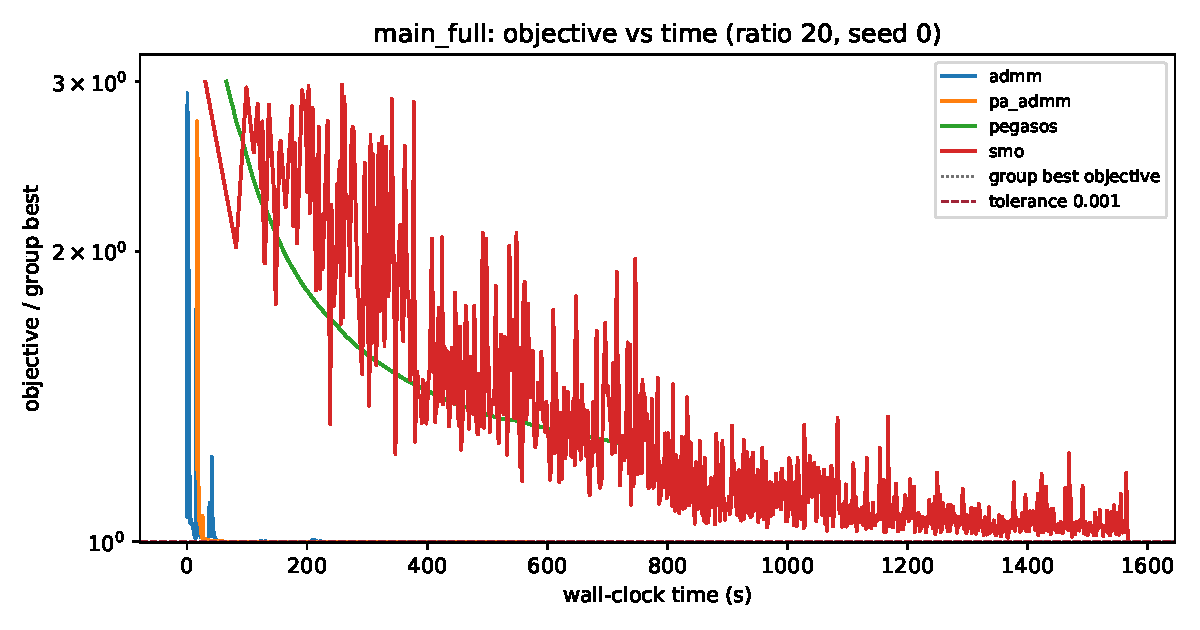
\includegraphics[width=\linewidth]{figures/archived_convergence.pdf}
\caption{Archived objective trajectories for the full-data experiment at ratio 20:1, seed 0. The vertical axis is objective divided by the group-best final value; the displayed range emphasizes the later part of optimization and omits larger initial values. The figure is reproduced from the project archive. SMO's primal objective can oscillate while it optimizes the dual. Precise target times and variation across all seeds are reported separately.}
\label{fig:convergence}
\end{figure}

The representative trajectory in Figure~\ref{fig:convergence} is compatible with the aggregate results: the ADMM variants approach the reference quickly, while the other two methods return less accurate primal solutions. SMO's primal oscillation should not be interpreted as monotonicity failure of its dual objective. The best measured primal checkpoint is retained for the returned model. The archived convergence figure is useful qualitative evidence, but one trajectory does not establish a convergence rate or a universal ordering.

\subsection{Does PA-ADMM improve the time to tolerance?}

Figure~\ref{fig:paired} shows all five paired target times, rather than only a favorable mean. At ratio 10:1, ADMM and PA-ADMM take $43.09\pm17.17$ and $44.40\pm13.43$ seconds. At 20:1, the corresponding values are $42.98\pm13.10$ and $49.20\pm11.79$ seconds. PA-ADMM has no average time advantage in these two settings. A warm start is not free, and it need not improve the initialization enough to repay its cost.

\begin{figure}[htbp]
\centering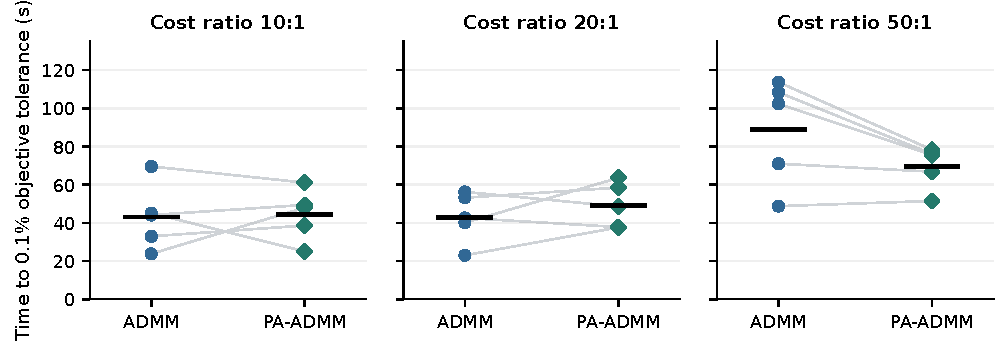
\includegraphics[width=\linewidth]{figures/paired_tolerance.pdf}
\caption{Full-data time to the common 0.1\% objective target. Gray segments connect the same seed; colored markers are individual runs; black horizontal marks show means. PA-ADMM times include the warm stage. All 30 plotted runs reach the target.}
\label{fig:paired}
\end{figure}

At ratio 50:1, PA-ADMM takes $69.60\pm11.05$ seconds, compared with $88.77\pm27.84$ seconds for ADMM. Their medians are 75.49 and 102.32 seconds: a descriptive 26.2\% median reduction. In medians, which is how the presentation reports these times, $T_\tau$ is 44.1 versus 47.9 seconds at 10:1, 42.6 versus 48.6 seconds at 20:1, and 102.3 versus 75.5 seconds at 50:1. The ordering reverses only at the harshest ratio, and the descriptive median reduction there is 26.2\%. The paired Wilcoxon $p$-values for 10:1, 20:1, and 50:1 are 1.0000, 0.4375, and 0.1250. The results therefore do not support a conventional significance claim. They suggest a potentially useful high-cost setting for further investigation, not an established general acceleration.

Total fit time tells a related but different story. At 10:1 and 20:1, PA-ADMM has higher mean total time; at 50:1, it has lower mean total time. Both ADMM implementations often continue hundreds of seconds after reaching the retrospective target. An early target crossing is consequently a measure of optimization progress, not the elapsed time a user would observe from the current solver's full call. A deployable early-stop rule would require a computable certificate or a separately justified stopping policy.

\subsection{Prediction quality and error cost}

Table~\ref{tab:prediction} reports the final models' test performance. AP is approximately 0.75--0.76 across the methods. The largest difference between mean AP values within a ratio is 0.0105 when Pegasos is included and 0.0035 among the three solvers that reach the common target, while sample standard deviations range from approximately 0.053 to 0.061. Recall at 1\% FPR is around 0.86--0.87. These observations do not establish a compelling predictive winner, but they also do not demonstrate statistical equivalence.

\begin{table}[htbp]
\caption{Full-data test results. AP and cost show mean $\pm$ sample standard deviation across five splits. Recall columns show means at 0.1\% and 1\% test FPR. Cost is multiplied by 1,000 for readability and uses the validation-selected threshold. Compare costs within a ratio.}
\label{tab:prediction}
\centering\small\setlength{\tabcolsep}{3.7pt}
\begin{tabular}{@{}llrrrr@{}}
\toprule
Cost & Solver & AP & Recall$_{0.1\%}$ & Recall$_{1\%}$ & Cost per 1,000\\
\midrule
10:1 & SMO & 0.749 $\pm$ 0.060 & 0.811 & 0.868 & 3.94 $\pm$ 0.68 \\
10:1 & Pegasos & 0.755 $\pm$ 0.059 & 0.842 & 0.868 & 3.41 $\pm$ 0.75 \\
10:1 & ADMM & 0.752 $\pm$ 0.055 & 0.831 & 0.868 & 3.80 $\pm$ 0.41 \\
10:1 & PA-ADMM & 0.752 $\pm$ 0.055 & 0.831 & 0.868 & 3.85 $\pm$ 0.46 \\
\addlinespace[3pt]
20:1 & SMO & 0.758 $\pm$ 0.059 & 0.834 & 0.870 & 6.81 $\pm$ 1.52 \\
20:1 & Pegasos & 0.756 $\pm$ 0.057 & 0.842 & 0.868 & 6.23 $\pm$ 1.43 \\
20:1 & ADMM & 0.760 $\pm$ 0.059 & 0.834 & 0.873 & 6.48 $\pm$ 1.41 \\
20:1 & PA-ADMM & 0.758 $\pm$ 0.061 & 0.834 & 0.873 & 6.51 $\pm$ 1.46 \\
\addlinespace[3pt]
50:1 & SMO & 0.761 $\pm$ 0.053 & 0.837 & 0.862 & 14.62 $\pm$ 3.42 \\
50:1 & Pegasos & 0.753 $\pm$ 0.055 & 0.837 & 0.870 & 14.47 $\pm$ 3.93 \\
50:1 & ADMM & 0.764 $\pm$ 0.055 & 0.837 & 0.870 & 14.62 $\pm$ 3.70 \\
50:1 & PA-ADMM & 0.764 $\pm$ 0.055 & 0.837 & 0.870 & 14.84 $\pm$ 3.84 \\
\bottomrule

\end{tabular}
\end{table}

The distinction between optimization and prediction is especially clear for Pegasos. Its training objective is substantially worse, yet at ratio 10:1 it has the lowest observed mean test cost, 0.003412 per transaction. ADMM's value is 0.003797 and PA-ADMM's is 0.003849. This does not make Pegasos the better optimizer; the objective and the test metric measure different quantities. Finite-sample ranking, regularization effects, and validation threshold selection can all separate their orderings. The current data do not identify which explanation dominates, and the small number of positives prevents a strong predictive-ranking claim.

\begin{figure}[htbp]
\centering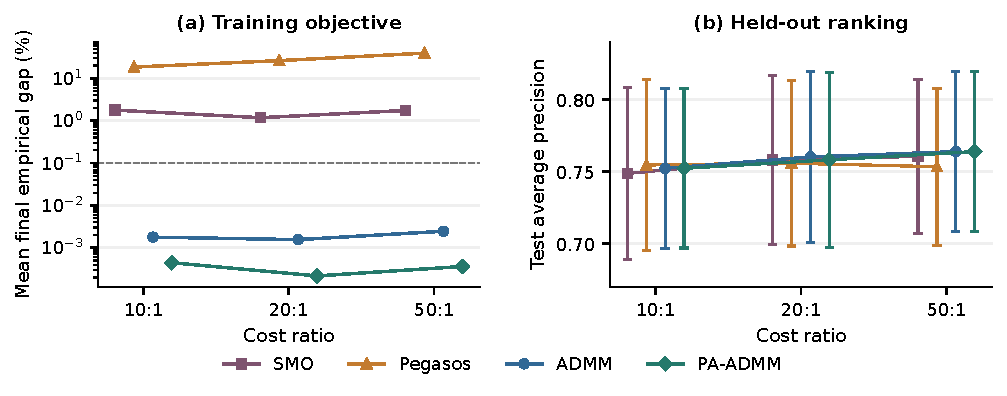
\includegraphics[width=\linewidth]{figures/objective_and_prediction.pdf}
\caption{Optimization accuracy and prediction should be read separately. Left: mean final empirical objective gap, on a logarithmic scale; the dashed line is the 0.1\% target. Right: mean test AP with sample-standard-deviation error bars. Large objective differences coexist with broadly similar held-out ranking results.}
\label{fig:quality}
\end{figure}

Every full-data test split has only 71 frauds. One additional detected fraud changes recall by approximately $1/71=1.41$ percentage points. At a 0.1\% FPR budget, only about 42 false alarms are permitted among the 42,488 legitimate test examples. These small counts help explain why both threshold-sensitive cost and low-FPR recall require careful interpretation. The stratified tests also do not represent a forward-in-time deployment evaluation.

\subsection{How the workload size changes the comparison}

Figure~\ref{fig:ladder} compares the small, medium, and full workloads at ratio 20:1. It reports total fit time together with final empirical gap, because a short capped run is not evidence of fast optimization to a common quality. The small correctness result already shows that SMO can be particularly efficient on a small instance. At the medium workload SMO still reaches the common target in two of three seeds, at a median 59.6 seconds against 12.4 seconds for ADMM, before exhausting its update cap; at the full scale no seed reaches it. All four methods complete every full workload inside the budget, Pegasos included, at a median of roughly twelve minutes, so the ladder separates methods by target attainment rather than by whether they finish. The ADMM variants' small dense linear solve makes them a good match for this dataset's low feature dimension.

\begin{figure}[htbp]
\centering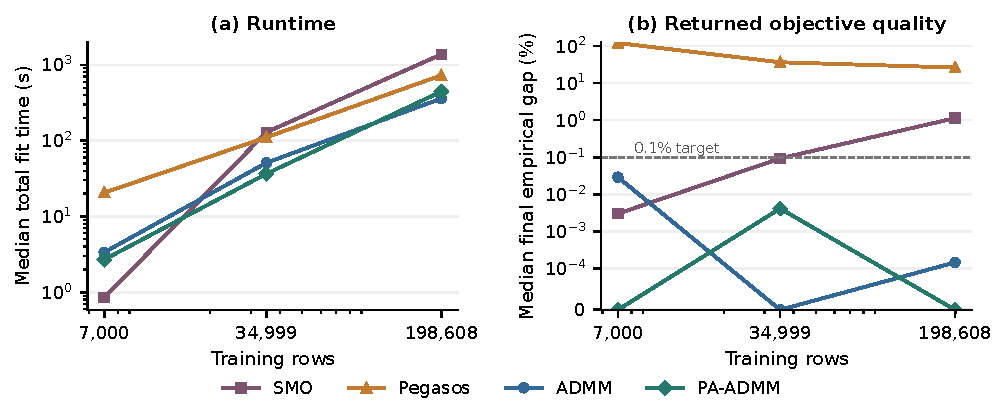
\includegraphics[width=\linewidth]{figures/size_ladder.pdf}
\caption{Observed workload ladder at ratio 20:1. Points are medians over three seeds for the smaller workloads and five for the full workload. The gap axis uses a symmetric logarithmic scale near zero. This is a comparison of completed workloads with fixed $C=1$ and configured caps, not a fitted asymptotic scaling law.}
\label{fig:ladder}
\end{figure}

The ladder has two important restrictions. First, the number of seeds changes from three to five. Second, holding $C=1$ in the unnormalized primal means the equivalent $\lambda=1/(nC)$ decreases as $n$ grows. Thus the workloads differ in statistical regularization as well as size. We do not infer a complexity exponent or a universal sample-size crossover from these points. A controlled scaling study would keep the relevant normalized regularization fixed and measure time to comparable optimization accuracy.

\section{Discussion and Limitations}

\paragraph{What the completed work establishes.}
The code implements four views of the same weighted linear SVM and checks that their returned objectives use the same convention. Independent numerical agreement on the small problem supports implementation consistency. On the full data, both ADMM variants reliably attain the shared empirical target under the tested settings, and PA-ADMM more often satisfies its own stopping conditions. The evidence also demonstrates that a large difference in training objective need not produce an equally large difference in held-out AP or operational cost.

\paragraph{What it does not establish.}
The main study has no completed unweighted $1{:}1$ training control evaluated at the same deployment cost. Therefore, it does not directly quantify the benefit of cost-sensitive training over an unweighted SVM. It does not isolate the PA components, prove a faster convergence rate, or show a universal best solver. A single low-dimensional dataset and three illustrative class-cost ratios are insufficient for those claims. Transaction-specific monetary losses are also not modeled: Amount is a feature, while the assumed cost matrix is class dependent.

\paragraph{Limits of the evidence.}
The repeated random splits overlap and are not a temporal holdout. The original proposal's noise, prevalence, and chronological checks remain unfinished. Method-specific caps can disadvantage an optimizer, and the common reference is computed from the same methods being compared. Missing CPU and RAM metadata limit independent interpretation of absolute times. The supplied archive retains detailed per-run CSV records, but not the raw transaction CSV or the per-iteration JSON logs used to make the original convergence curve. These omissions limit artifact-only verification of the trajectories, although the aggregate tables can be independently recomputed.

\paragraph{Priorities for further work.}
The most informative next experiment is a matched ADMM ablation: cold fixed-$\rho$, cold adaptive-$\rho$, warm adaptive-$\rho$ without relaxation, and the full PA variant. It should charge initialization time and report both an empirical target and solver certificates. An unweighted training control should be evaluated under each fixed deployment cost to isolate the value of class weighting. Chronological evaluation and larger numbers of positive test cases would strengthen predictive claims. Finally, tuning the stochastic schedule and comparing a mature linear SVM solver would test whether the present Pegasos and SMO outcomes mainly reflect the chosen implementations and budgets.

\section{Conclusions}

We formulated credit card fraud detection as a cost-sensitive convex SVM and implemented SMO, weighted Pegasos, ADMM, and PA-ADMM under a common objective. The completed experiments favor ADMM-based optimization for the tested large-$n$, small-$d$ linear setting: both variants reach the empirical target on all full-data runs. PA-ADMM improves the observed completion of its internal stopping rule, but its additional initialization does not consistently reduce time, and the five-seed comparison does not establish statistical superiority. SMO performs well on the small correctness problem but is limited by its configured update cap at full scale. Pegasos shows that a less accurate training solution can still provide comparable held-out ranking quality. The main practical lesson is to report objective quality, elapsed time, stopping evidence, and application cost together, while keeping the model and evaluation protocol fixed.

\section*{Reproducibility and artifact notes}

{\raggedright
The implementation and experiment configuration are in the supplied project archive. \texttt{EXPERIMENTS.md} documents data preparation and execution; \texttt{docs/INTERFACES.md} specifies the solver contract. The report uses four completed per-run CSVs in \texttt{results/tables}:\par
{\small\ttfamily correctness\_runs.csv, main\_capped\_runs.csv,\\
main\_fast\_runs.csv, main\_full\_runs.csv.}\par
The full-data summary and Wilcoxon CSVs supply the archived aggregates and paired tests. These records take precedence over earlier proposal settings and preliminary slide summaries.\par}

To reproduce training, obtain \texttt{creditcard.csv} from the documented dataset source, place it in \texttt{data/raw}, and verify the raw shape of 284,807 rows and 31 columns, including 492 positive labels. Run commands from the project root:
\begin{Verbatim}[fontsize=\small]
python -m pip install -r requirements.txt
python -m pytest -q
python experiments/run_correctness.py --config configs/correctness.yaml
python experiments/run_main.py --config configs/main_capped.yaml
python experiments/run_main.py --config configs/main_fast.yaml
python experiments/run_main.py --config configs/main_full.yaml
\end{Verbatim}
The saved split indices refer to the deduplicated, reset-index dataset, not the raw CSV. Existing matching runs may be reused by the harness; use the documented overwrite setting when a complete refit is required. The 90-minute allowance is per fit, so these commands should not be interpreted as a short smoke test. Package requirements are lower bounds, not a fully locked environment.

As a separate verification during report preparation, 112 existing tests covering SMO, Pegasos, ADMM, the solver interface, and metrics passed on the supplied source. No full-data benchmark was rerun for this report. The accompanying report source includes the original per-run CSVs used here and a script to regenerate its new tables and aggregate figures. The archived convergence PDF is included unchanged; regenerating that curve requires the original trajectory logs or fresh runs.

\section*{Writing assistance}
Generative AI assisted with organizing and drafting this report, checking consistency between the provided source code and experiment tables, and preparing figures and \LaTeX{} formatting. Reported ULB benchmark results come from the group's archived experiments; additional large-scale results have not been generated or inferred.

\FloatBarrier
\begin{thebibliography}{10}
\small\raggedright
\bibitem[Cortes and Vapnik(1995)]{cortes1995}
C. Cortes and V. Vapnik.
Support-vector networks.
\emph{Machine Learning}, 20:273--297, 1995.
\href{https://doi.org/10.1007/BF00994018}{doi:10.1007/BF00994018}.

\bibitem[Elkan(2001)]{elkan2001}
C. Elkan.
The foundations of cost-sensitive learning.
In \emph{Proceedings of the 17th International Joint Conference on Artificial Intelligence}, pp.\ 973--978, 2001.
\url{https://cseweb.ucsd.edu/~elkan/rescale.pdf}.

\bibitem[Platt(1998)]{platt1998}
J. C. Platt.
Sequential minimal optimization: A fast algorithm for training support vector machines.
Technical Report MSR-TR-98-14, Microsoft Research, 1998.
\url{https://www.microsoft.com/en-us/research/wp-content/uploads/2016/02/tr-98-14.pdf}.

\bibitem[Fan et~al.(2005)]{fan2005}
R.-E. Fan, P.-H. Chen, and C.-J. Lin.
Working set selection using second order information for training support vector machines.
\emph{Journal of Machine Learning Research}, 6:1889--1918, 2005.
\url{https://jmlr.org/papers/v6/fan05a.html}.

\bibitem[Chang and Lin(2011)]{chang2011}
C.-C. Chang and C.-J. Lin.
LIBSVM: A library for support vector machines.
\emph{ACM Transactions on Intelligent Systems and Technology}, 2(3), Article 27, 2011.
\href{https://doi.org/10.1145/1961189.1961199}{doi:10.1145/1961189.1961199}.

\bibitem[Shalev-Shwartz et~al.(2011)]{shalev2011}
S. Shalev-Shwartz, Y. Singer, N. Srebro, and A. Cotter.
Pegasos: Primal estimated sub-gradient solver for SVM.
\emph{Mathematical Programming}, 127:3--30, 2011.
\href{https://doi.org/10.1007/s10107-010-0420-4}{doi:10.1007/s10107-010-0420-4}.

\bibitem[Boyd et~al.(2011)]{boyd2011}
S. Boyd, N. Parikh, E. Chu, B. Peleato, and J. Eckstein.
Distributed optimization and statistical learning via the alternating direction method of multipliers.
\emph{Foundations and Trends in Machine Learning}, 3(1):1--122, 2011.
\href{https://doi.org/10.1561/2200000016}{doi:10.1561/2200000016}.

\bibitem[Boyd and Vandenberghe(2004)]{boyd2004}
S. Boyd and L. Vandenberghe.
\emph{Convex Optimization}.
Cambridge University Press, 2004.
\url{https://web.stanford.edu/~boyd/cvxbook/}.

\bibitem{ulb}
ULB Machine Learning Group and Worldline.
Credit Card Fraud Detection dataset.
Kaggle, transactions collected in September 2013.
\url{https://www.kaggle.com/datasets/mlg-ulb/creditcardfraud}.

\bibitem[scikit-learn developers(2026)]{sklearnap}
scikit-learn developers.
\texttt{average\_precision\_score}: API reference and metric definition.
\url{https://scikit-learn.org/stable/modules/generated/sklearn.metrics.average_precision_score.html}.
Accessed 30 October 2026.
\end{thebibliography}
\end{document}
